\documentclass{standalone}
\usepackage{tikz}
\begin{document}
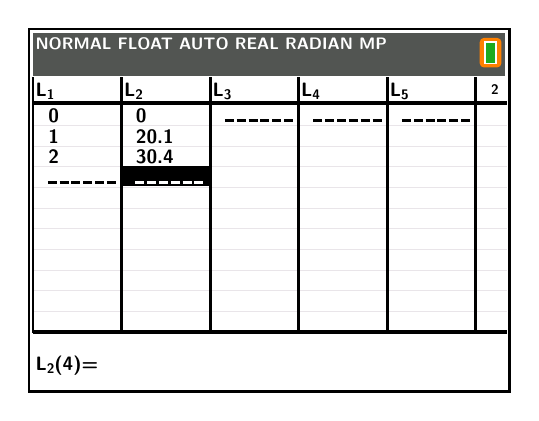
\begin{tikzpicture}[x=0.025cm, y=-0.025cm, font=\sffamily\bfseries]
  % TI-84 Plus CE list editor screen (1 unit = 1 screen pixel, y downward)
  \definecolor{tibar}{RGB}{82,85,82}
  \definecolor{tigrid}{RGB}{233,229,233}
  \definecolor{tiorange}{RGB}{255,128,0}
  \definecolor{tigreen}{RGB}{31,170,31}
  % Screen border
  \draw[line width=1pt] (0,0) rectangle (244,184);
  % Status bar
  \fill[tibar] (2,2) rectangle (242,24);
  \node[anchor=west, white, font=\sffamily\bfseries\fontsize{6.4}{7}\selectfont, inner sep=0]
    at (3,7.5) {NORMAL FLOAT AUTO REAL RADIAN MP};
  % Battery icon
  \fill[tiorange, rounded corners=1.5] (229,4.5) rectangle (240,19.5);
  \fill[white] (231,6) rectangle (238,18);
  \fill[tigreen] (232,7) rectangle (237,17);
  % Light row gridlines
  \foreach \y in {49,59.5,70,80.5,91,101.5,112,122.5,133,143.5}
    \draw[tigrid, line width=0.4pt] (2,\y) -- (243,\y);
  % Highlighted (cursor) cell: L2, row 4
  \fill[black] (47,69.5) rectangle (92,79.5);
  % Table lines
  \draw[line width=1pt] (2,24.5) -- (2,154.5);
  \foreach \x in {47,92,137,182,227}
    \draw[line width=1pt] (\x,24.5) -- (\x,154.5);
  \draw[line width=1.2pt] (2,37.5) -- (243,37.5);
  \draw[line width=1.2pt] (2,154) -- (243,154);
  % Column headers
  \foreach \x/\n in {3/1,48/2,93/3,138/4,183/5}
    \node[anchor=west, inner sep=0, font=\sffamily\bfseries\scriptsize]
      at (\x,31.5) {L\raisebox{-0.35ex}{\tiny\n}};
  \node[anchor=west, inner sep=0, font=\sffamily\bfseries\tiny]
    at (234.5,31) {2};
  % L1 entries
  \foreach \y/\v in {44/0,54.5/1,65/2}
    \node[anchor=west, inner sep=0, font=\sffamily\bfseries\scriptsize]
      at (9.5,\y) {\v};
  % L2 entries
  \foreach \y/\v in {44/0,54.5/20.1,65/30.4}
    \node[anchor=west, inner sep=0, font=\sffamily\bfseries\scriptsize]
      at (54,\y) {\v};
  % End-of-list dashes ("------")
  % (dash lengths in pt: 1 screen pixel = 0.025cm = 0.71pt)
  \tikzset{tidash/.style={line width=1pt, dash pattern=on 3.27pt off 1pt}}
  \draw[tidash] (9.5,78) -- ++(34.6,0);
  \draw[tidash, white] (54,78) -- ++(34.6,0);
  \draw[tidash] (99.5,46.5) -- ++(34.6,0);
  \draw[tidash] (144.5,46.5) -- ++(34.6,0);
  \draw[tidash] (189.5,46.5) -- ++(34.6,0);
  % Entry line
  \node[anchor=west, inner sep=0, font=\sffamily\bfseries\scriptsize]
    at (3,171) {L\raisebox{-0.35ex}{\tiny 2}(4)=};
\end{tikzpicture}
\end{document}
